% Preamble templated from Mihir-Divyansh/Course-Setup
%iffalse
\let\negmedspace\undefined
\let\negthickspace\undefined
\documentclass[journal,12pt,onecolumn]{IEEEtran}
\usepackage{cite}
\usepackage{amsmath,amssymb,amsfonts,amsthm}
\usepackage{algorithmic}
\usepackage{graphicx}
\usepackage{textcomp}
\usepackage{xcolor}
\usepackage{txfonts}
\usepackage{listings}
\usepackage{enumitem}
\usepackage{mathtools}
\usepackage{gensymb}
\usepackage{comment}
\usepackage[breaklinks=true]{hyperref}
\usepackage{tkz-euclide}
\usepackage{listings}
\usepackage{gvv}
%\def\inputGnumericTable{}
\usepackage[latin1]{inputenc}
\usepackage{color}
\usepackage{array}
\usepackage{longtable}
\usepackage{calc}
\usepackage{multirow}
\usepackage{hhline}
\usepackage{ifthen}
\usepackage{lscape}
\usepackage{tabularx}
\usepackage{array}
\usepackage{float}
\usepackage{caption}
\usepackage{multicol}

\newtheorem{theorem}{Theorem}[section]
\newtheorem{problem}{Problem}
\newtheorem{proposition}{Proposition}[section]
\newtheorem{lemma}{Lemma}[section]
\newtheorem{corollary}[theorem]{Corollary}
\newtheorem{example}{Example}[section]
\newtheorem{definition}[problem]{Definition}
\newcommand{\BEQA}{\begin{eqnarray}}
\newcommand{\EEQA}{\end{eqnarray}}
%\newcommand{\define}{\stackrel{\triangle}{=}}
\theoremstyle{remark}
%\newtheorem{rem}{Remark}

% Marks the beginning of the document
\begin{document}
\bibliographystyle{IEEEtran}
\vspace{3cm}

\title{Assignment 8: 4.11.32}
\author{EE25BTECH11055 - Subhodeep Chakraborty}
\maketitle
\hrulefill
\bigskip

\renewcommand{\thefigure}{\theenumi}
\renewcommand{\thetable}{\theenumi}

\textbf{Question:}\par
Find the equation of the line passing through \brak{2,-1,2} and \brak{5,3,4} and of the plane passing through \brak{2,0,3}, \brak{1,1,5} and \brak{3,2,4}. Also, find their point of intersection. \hfill \brak{12,2018}
\par
\textbf{Solution:}\par

Given:
\begin{align}
 \vec{A} &= \myvec{2\\-1\\2} \\
 \vec{B} &= \myvec{5\\3\\4} \\
 \vec{P} &= \myvec{2\\0\\3} \\
 \vec{Q} &= \myvec{1\\1\\5} \\
 \vec{R} &= \myvec{3\\2\\4}
\end{align}

We know, for line $\vec{x} = \vec{h} +k\vec{m}$ and plane $\vec{n}^\top\vec{y}=1$,
\begin{align}
 \vec{h} &= \vec{A} \\
 \vec{m} &= \vec{B-A} \\
 \myvec{P & Q & R}^\top\vec{n} &= \myvec{1\\1\\1} \\
 \text{Also, for intersection}\\
 \vec{x}=\vec{y} \implies \vec{n}^\top\brak{\vec{h}+k\vec{m}} = 1\\
 k = \frac{1-\vec{n}^\top\vec{h}}{\vec{n}^\top\vec{m}} \\
 \vec{x} = \vec{h} + \brak{\frac{1-\vec{n}^\top\vec{h}}{\vec{n}^\top\vec{m}}}\vec{m}
\end{align}
Thus
\begin{align}
  \myvec{P & Q & R}^\top\vec{n} &= \myvec{1\\1\\1} \\
  \myvec{2 & 0 & 3 \\ 1 & 1 & 5 \\ 3 & 2 & 4}\vec{n} &= \myvec{1\\1\\1}
\end{align}
\begin{align}
  \augvec{3}{1}{2 & 0 & 3 & 1 \\ 1 & 1 & 5 & 1\\ 3 & 2 & 4 & 1} &\xleftrightarrow[]{R_2 = 2R_2-R_1; R_3 = 2R_3-3R_1}
  \augvec{3}{1}{2 & 0 & 3 & 1 \\ 0 & 2 & 7 & 1\\ 0 & 4 & 2 & -1} \\ \xleftrightarrow[]{R_3=R_3-2R_2}
  \augvec{3}{1}{2 & 0 & 3 & 1 \\ 0 & 2 & 7 & 1\\ 0 & 0 & -12 & -3} &\xleftrightarrow[]{R_1=4R_1+R_3; R_2= 12R_2+7R_3}
  \augvec{3}{1}{8 & 0 & 0 & 1 \\ 0 & 24 & 0 & -9 \\ 0 & 0 & -12 & -3} \\ &\xleftrightarrow[]{R_1 = R_1/8; R_2 = R_2/24; R_3 = -R_3/12}
  \augvec{3}{1}{1 & 0 & 0 & 1/8 \\ 0 & 1 & 0 & -3/8 \\ 0 & 0 & 1 & 1/4} \\
  \vec{n} &= \frac{1}{8}\myvec{1\\-3\\2}
\end{align}
So we have:
\begin{align}
\vec{n}^\top\vec{h}= \frac{1}{8}\myvec{1&-3&2}\myvec{2\\-1\\2} = \frac{9}{8}\\
\vec{n}^\top\vec{m} = \frac{1}{8}\myvec{1&-3&2}\myvec{3\\4\\2} = -\frac{5}{8} \\
\vec{x} = \myvec{2\\-1\\2} + \brak{\frac{1-9/8}{-5/8}}
\myvec{3\\4\\2} = \myvec{13/5\\-1/5\\12/5 }
\end{align}
\begin{figure}[H]
    \centering
    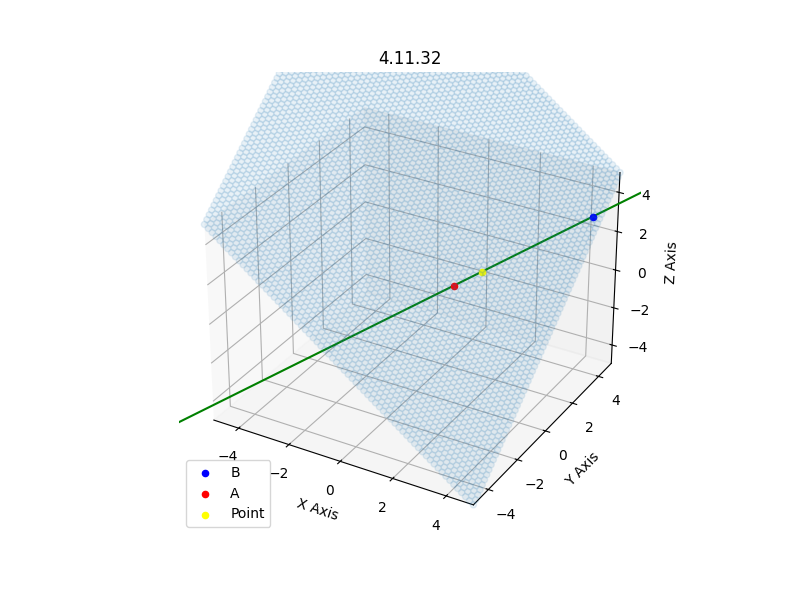
\includegraphics{figs/plot.png}
    \caption*{}
    \label{fig:plot}
\end{figure}
\end{document}
